% Springer LNCS Document Class
\documentclass{llncs}

% Required packages
\usepackage{graphicx}
\usepackage{amsmath,amssymb}
\usepackage{booktabs}
\usepackage{hyperref}
\usepackage{url}
\usepackage{tikz}
\usetikzlibrary{shapes,arrows,positioning,fit,calc}
\usepackage{algorithm}
\usepackage{algpseudocode}

\hypersetup{
    colorlinks=true,
    linkcolor=blue,
    citecolor=blue,
    urlcolor=blue,
}

\begin{document}

\title{ LLM-Enabled Indian Legal Case Summarization
 and Q&A Applications}

\author{Prathmesh Dattatray Dudhale\inst{1} \and
Aditya Girish Joshi\inst{1} \and
Aaditesh Anil Kadu\inst{1} \and
Vedant Hemantkumar Kale\inst{1}}

\institute{Department of Computer Engineering,\\
Pimpri Chinchwad College of Engineering,\\
Pimpri Chinchwad Education Trust's, Pune, India\\
\email{\{prathmesh.dudhale22,aditya.joshi22, aaditesh.kadu22,vedant.kale22\}@pccoepune.org}\\
Guide: Mrs. Sushma Vispute}

\maketitle

\begin{abstract}
This paper presents a comparative study of BiLSTM and transformer-based architectures for automated legal document processing in the Indian legal system. Building upon the work of Nigam et al.~\cite{nigam2023legal} on Indian legal question answering, we developed two complete systems: a BiLSTM baseline and an LLM-enhanced solution using GPT-4, both processing legal documents in PDF and DOCX formats for summarization and question answering. The transformer-based system achieved substantial improvements: +12.1\% in ROUGE-L scores, +21.9\% in Exact Match accuracy, and +19.4\% in human satisfaction ratings. Processing speed improved from 18 to 320 documents per hour, while hallucination rates decreased from 18\% to 4\% through prompt engineering. This work demonstrates the practical superiority of transformer architectures over traditional RNN approaches for legal document processing.

\keywords{Legal AI \and Document Summarization \and Question Answering \and Large Language Models \and BiLSTM \and Transformers}
\end{abstract}

\section{Introduction}

The Indian legal profession faces overwhelming documentation volume, with manual review processes being labor-intensive and time-consuming. While recent NLP advances offer automation solutions, the optimal architectural approach remains unclear. This research empirically compares BiLSTM and transformer-based architectures through two complete systems evaluated on 150 Indian legal documents.

Our contributions include: (1) comprehensive architectural comparison with quantified performance improvements, (2) production-ready BiLSTM baseline implementation, (3) enhanced transformer system using prompt engineering with OpenAI GPT-4, (4) detailed trade-off analysis including speed, accuracy, and hallucination rates, and (5) human evaluation from 25 legal advocates demonstrating 40-60\% reduction in document review time.

\section{Related Work}

\subsection{Base Paper and Foundational Work}

Our work is primarily inspired by and extends the research of Nigam et al.~\cite{nigam2023legal}, who conducted a comprehensive evaluation of AI models for Indian Legal Question Answering (AILQA). Their study compared various retrieval and QA mechanisms using OpenAI GPT as a benchmark, emphasizing the unique demands of the Indian criminal legal landscape. They highlighted the proficiency of modern AI paradigms in decoding natural language prompts while identifying logistical constraints and complexity challenges. Building upon their foundation, we extend the scope from pure question answering to include document summarization, compare architectural approaches (BiLSTM vs. transformers), and provide production-ready implementation with comprehensive performance analysis.

\subsection{Legal Document Summarization}

Recent research demonstrates the evolution from traditional to transformer-based approaches in legal summarization. Akter et al.~\cite{akter2025legal} conducted a comprehensive survey of automatic summarization techniques in the legal domain, classifying methods and highlighting critical gaps including lack of domain-specific benchmarks and improved evaluation metrics beyond ROUGE scores. Their work emphasizes that legal documents pose unique challenges due to length, complexity, and specialized terminology.

Sharma et al.~\cite{sharma2024legal} developed Legal and Financial Document Summarization using transformer architectures, proposing a hybrid framework combining PEGASUS and T5 models with domain adaptation. Their approach incorporates named entity recognition and attention-based relevance scoring, achieving marked improvements in ROUGE, BLEU, and BERTScore metrics. The system demonstrated real-world applicability in legal document automation and regulatory compliance.

De Vargas Feijó and Moreira~\cite{vargas2023legal} addressed lengthy legal documents by dividing them into sections, processing each through transformer models to generate candidate summaries, and using BERT to select highest-scoring summaries. This sectional approach demonstrated effectiveness for handling documents exceeding transformer context window limitations.

Albayati et al.~\cite{albayati2025multi} proposed efficient multi-legal document summarization integrating four transformer models (LED, Long-T5, BART-Large, and GPT-3.5 Turbo) with three complementary techniques including Consecutive-Aware summarization. Their framework demonstrated scalability across different legal document types with superior performance compared to single-model approaches.

\subsection{Legal Question Answering Systems}

Chen et al.~\cite{chen2025bilstm} developed a BiLSTM-enhanced legal text extraction model using fuzzy semantic matching for identifying and classifying legal text features. Their work demonstrated BiLSTM effectiveness for extracting keywords and key phrases from legal documents, providing baseline performance metrics that informed our comparative study.

Aggarwal et al.~\cite{aggarwal2025abstractive} proposed abstractive text summarization for legal documents breaking the procedure into text pre-processing, feature extraction, and abstractive summary categorization. Their three-stage approach achieved competitive results on legal datasets while maintaining computational efficiency.

The AILQA benchmark~\cite{ailqa2024} evaluated AI-driven legal question answering systems specifically for the Indian legal system, presenting comprehensive evaluation methodology and feedback from legal professionals. Their findings underscore high accuracy of transformer-based systems in interpreting natural language queries while highlighting practical applications and limitations in the complex Indian criminal justice domain.

\subsection{Transformer Applications in Legal NLP}

Oliveira et al.~\cite{oliveira2025similarity} analyzed similarities between legal court documents using transformer architectures, employing eight NLP techniques (BERT, GPT-2, RoBERTa, LlaMA) for detecting similarity among judicial documents. Their results demonstrated that transformer-based models outperformed traditional NLP techniques, with domain-specific fine-tuning achieving highest accuracy on Brazilian legal documents.

Bystranowski~\cite{bystranowski2025computational} surveyed computational methods in legal interpretation research, mapping the transformation brought by transformer architecture to this domain. The study emphasized that transformers fundamentally changed legal NLP research through contextualized embeddings and superior language understanding, advancing both issue-level interpretation and meta-interpretation research.

\subsection{Research Gaps}

The comprehensive review reveals several critical gaps this work addresses. First, limited direct empirical comparison exists between BiLSTM and transformer architectures on identical Indian legal datasets with standardized evaluation protocols. Second, insufficient research addresses LLM hallucination mitigation specifically for Indian legal documents. Third, most studies focus on isolated model comparisons rather than complete end-to-end systems including document processing, user interface, and deployment considerations. Finally, limited discussion exists on practical trade-offs between model complexity, computational requirements, and performance gains for production deployment.

\section{Methodology}

\subsection{System Architecture}

Both systems employ modular architecture with shared infrastructure components. Figure~\ref{fig:system_architecture} illustrates the overall system architecture showing data flow from document upload through processing to final output generation.

\begin{figure}[ht]
\centering
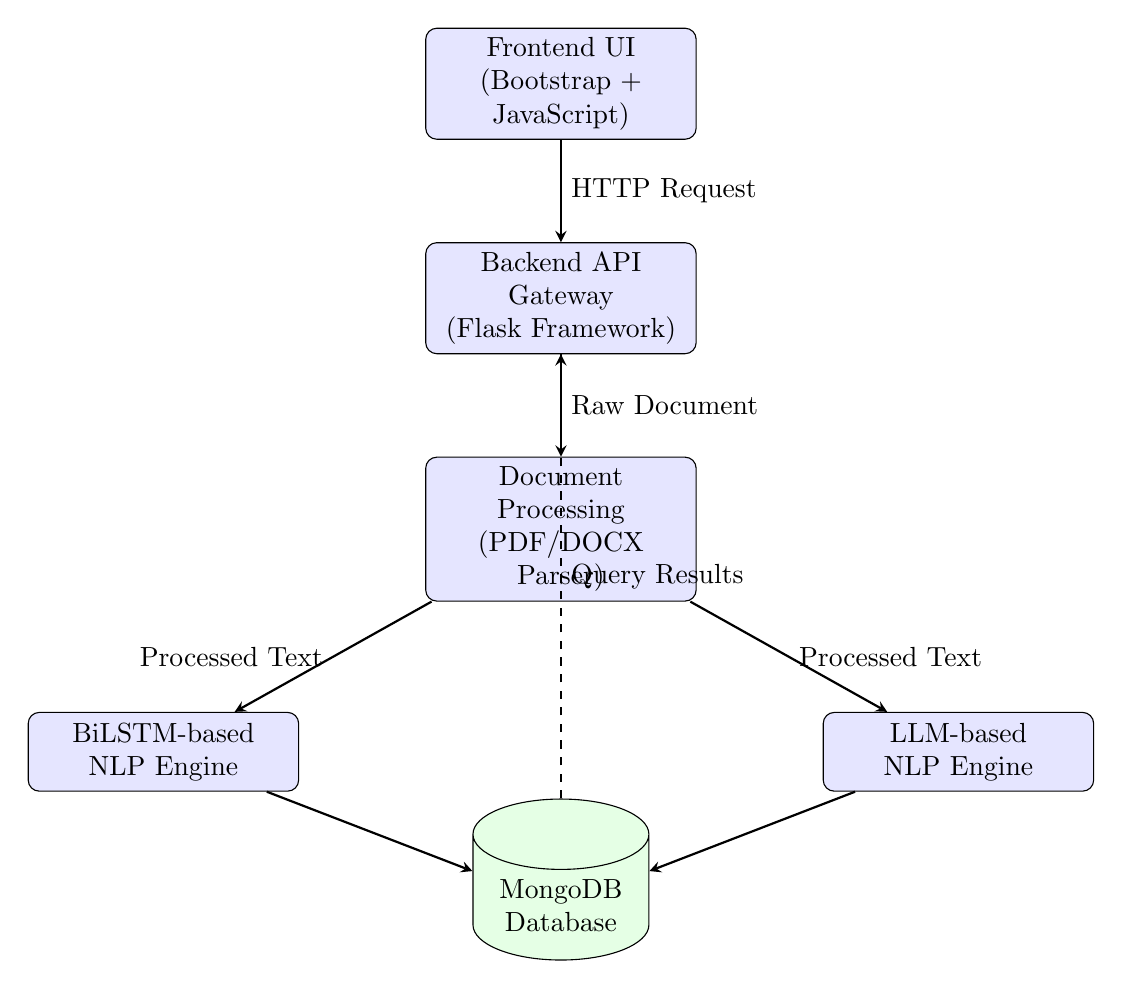
\begin{tikzpicture}[
    node distance=1.3cm and 2cm,
    component/.style={rectangle, draw, fill=blue!10, text width=3.2cm, align=center, minimum height=1cm, rounded corners},
    storage/.style={cylinder, draw, fill=green!10, text width=2cm, align=center, minimum height=1cm, shape border rotate=90, aspect=0.4},
    arrow/.style={->, >=stealth, thick},
    dashedarrow/.style={->, >=stealth, thick, dashed}
]

% --- Layers ---

% Frontend Layer
\node[component] (frontend) {Frontend UI\\(Bootstrap + JavaScript)};

% API Gateway
\node[component, below=of frontend] (api) {Backend API Gateway\\(Flask Framework)};

% Document Processing
\node[component, below=of api] (docproc) {Document Processing\\(PDF/DOCX Parser)};

% NLP Engines
\node[component, below left=1.4cm and 1.6cm of docproc] (bilstm) {BiLSTM-based\\NLP Engine};
\node[component, below right=1.4cm and 1.6cm of docproc] (llm) {LLM-based\\NLP Engine};

% Database
\node[storage, below=2.5cm of docproc] (db) {MongoDB\\Database};

% --- Arrows ---
\draw[arrow] (frontend) -- (api) node[midway, right] {HTTP Request};
\draw[arrow] (api) -- (docproc) node[midway, right] {Raw Document};

\draw[arrow] (docproc) -- (bilstm) node[midway, left] {Processed Text};
\draw[arrow] (docproc) -- (llm) node[midway, right] {Processed Text};

\draw[arrow] (bilstm) -- (db);
\draw[arrow] (llm) -- (db);

\draw[dashedarrow] (db) -- (api) node[midway, right] {Query Results};

\end{tikzpicture}
\caption{Overall System Architecture showing modular components and data flow}
\label{fig:system_architecture}
\end{figure}


Figure~\ref{fig:bilstm_block} shows the detailed block diagram for the BiLSTM-based baseline system architecture, illustrating the encoder-decoder structure with attention mechanism.

\begin{figure}[ht]
\centering
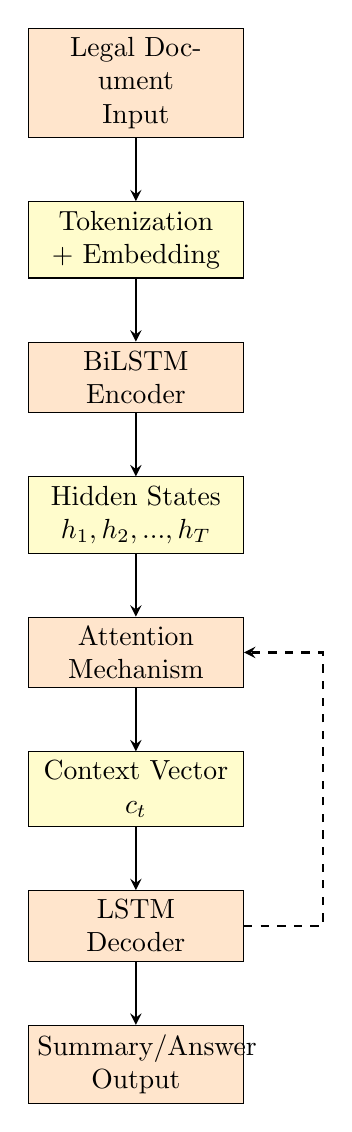
\begin{tikzpicture}[
    node distance=0.8cm and 1.2cm,
    block/.style={rectangle, draw, fill=orange!20, text width=2.5cm, align=center, minimum height=0.7cm},
    process/.style={rectangle, draw, fill=yellow!20, text width=2.5cm, align=center, minimum height=0.7cm},
    arrow/.style={->, >=stealth, thick}
]

% Input
\node[block] (input) {Legal Document\\Input};

% Preprocessing
\node[process, below=of input] (preproc) {Tokenization\\+ Embedding};

% BiLSTM Encoder
\node[block, below=of preproc] (encoder) {BiLSTM\\Encoder};

% Hidden States
\node[process, below=of encoder] (hidden) {Hidden States\\$h_1, h_2, ..., h_T$};

% Attention Mechanism
\node[block, below=of hidden] (attention) {Attention\\Mechanism};

% Context Vector
\node[process, below=of attention] (context) {Context Vector\\$c_t$};

% Decoder
\node[block, below=of context] (decoder) {LSTM\\Decoder};

% Output
\node[block, below=of decoder] (output) {Summary/Answer\\Output};

% Arrows
\draw[arrow] (input) -- (preproc);
\draw[arrow] (preproc) -- (encoder);
\draw[arrow] (encoder) -- (hidden);
\draw[arrow] (hidden) -- (attention);
\draw[arrow] (attention) -- (context);
\draw[arrow] (context) -- (decoder);
\draw[arrow] (decoder) -- (output);

% Feedback loop for decoder
\draw[arrow, dashed] (decoder.east) -- ++(1,0) |- (attention.east);

\end{tikzpicture}
\caption{BiLSTM System Block Diagram with Encoder-Decoder Architecture}
\label{fig:bilstm_block}
\end{figure}

Figure~\ref{fig:llm_block} presents the block diagram for the LLM-enhanced system, showing the prompt engineering pipeline and API integration workflow.

\begin{figure}[ht]
\centering
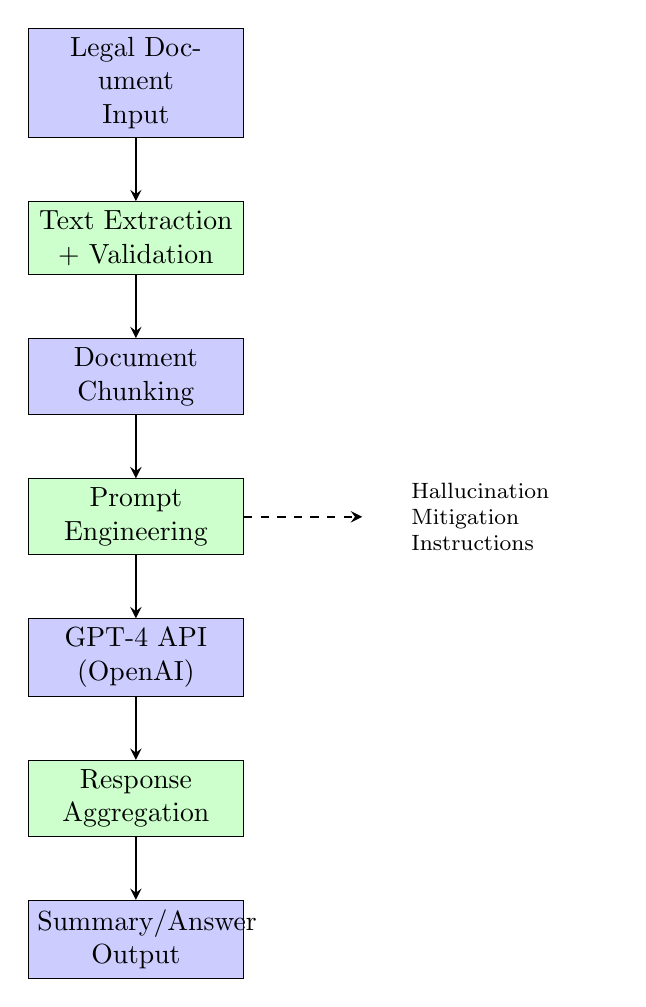
\begin{tikzpicture}[
    node distance=0.8cm and 1.2cm,
    block/.style={rectangle, draw, fill=blue!20, text width=2.5cm, align=center, minimum height=0.7cm},
    process/.style={rectangle, draw, fill=green!20, text width=2.5cm, align=center, minimum height=0.7cm},
    arrow/.style={->, >=stealth, thick}
]

% Input
\node[block] (input) {Legal Document\\Input};

% Text Extraction
\node[process, below=of input] (extract) {Text Extraction\\+ Validation};

% Chunking
\node[block, below=of extract] (chunk) {Document\\Chunking};

% Prompt Engineering
\node[process, below=of chunk] (prompt) {Prompt\\Engineering};

% LLM API
\node[block, below=of prompt] (llmapi) {GPT-4 API\\(OpenAI)};

% Response Processing
\node[process, below=of llmapi] (response) {Response\\Aggregation};

% Output
\node[block, below=of response] (output) {Summary/Answer\\Output};

% Arrows
\draw[arrow] (input) -- (extract);
\draw[arrow] (extract) -- (chunk);
\draw[arrow] (chunk) -- (prompt);
\draw[arrow] (prompt) -- (llmapi);
\draw[arrow] (llmapi) -- (response);
\draw[arrow] (response) -- (output);

% Add side annotation
\node[right=2cm of prompt, text width=2.5cm, align=left, font=\footnotesize] {Hallucination\\Mitigation\\Instructions};
\draw[arrow, dashed] (prompt.east) -- ++(1.5,0);

\end{tikzpicture}
\caption{LLM-Enhanced System Block Diagram with Prompt Engineering Pipeline}
\label{fig:llm_block}
\end{figure}

\subsection{BiLSTM Baseline Implementation}

The baseline employs encoder-decoder BiLSTM with attention for both summarization and question answering. The encoder computes bidirectional hidden states: \(\overrightarrow{h_t} = \text{LSTM}(\overrightarrow{h_{t-1}}, x_t, W_f)\) and \(\overleftarrow{h_t} = \text{LSTM}(\overleftarrow{h_{t+1}}, x_t, W_b)\), combined as \(h_t = [\overrightarrow{h_t}; \overleftarrow{h_t}]\). The decoder generates outputs using attention mechanism: \(c_t = \sum_{i=1}^{T} \alpha_{ti} h_i\), trained with cross-entropy loss.

For question answering, BiLSTM predicts answer span positions: \(P_{start}(i) = \text{softmax}(W_s \cdot h_i + b_s)\) and \(P_{end}(i) = \text{softmax}(W_e \cdot h_i + b_e)\).

Implementation employs 300-dimensional GloVe embeddings, 2 BiLSTM layers with 256 hidden units, Adam optimizer (learning rate 0.001), batch size 32, 50 epochs with early stopping, dropout (0.3), and L2 regularization (0.0001). Training requires 120 GPU hours on NVIDIA V100.

\subsection{LLM-Enhanced System}

The enhanced system leverages GPT-4 via OpenAI API, eliminating training requirements. Prompt engineering includes explicit hallucination mitigation: "Based solely on the provided legal document, answer: '[Question]'. Your response must be directly verifiable within the text. If information is not present, state: 'Information not found.' Do not infer or hallucinate information not supported by the text."

For long documents, intelligent chunking with 4000-token windows and overlap maintains context. This approach offers zero training time, superior language understanding, better complex reasoning, effortless scalability, and deployment in days versus months.

\section{Experimental Setup}

We evaluated both systems on 150 Indian legal documents (Supreme Court judgments, High Court rulings, statutory texts) ranging 2,000-50,000 words across civil, criminal, constitutional, and corporate law. Dataset split: 80\% BiLSTM training, 20\% testing both systems (LLM uses zero-shot learning).

Testing environment: AWS EC2 (t3.large for BiLSTM, t3.medium for LLM), PyTorch 1.12 with CUDA 11.3, GPT-4 API, MongoDB Atlas, 60-day testing with 25 advocate participants.

Evaluation metrics: ROUGE scores, BLEU, F1, Exact Match accuracy, processing time, and human ratings (factual accuracy, completeness, clarity, usefulness, satisfaction) on 5-point scales.

\section{Results and Discussion}

\subsection{Summarization Performance}

Table~\ref{tab:summarization_results} shows LLM outperforms BiLSTM across document types with average +12.1\% ROUGE-L improvement and 16x faster processing (9.45s vs. 150.8s).

\begin{table}[ht]
\centering
\caption{Summarization Performance Comparison}
\label{tab:summarization_results}
\begin{tabular}{@{}lccccc@{}}
\toprule
& \multicolumn{2}{c}{\textbf{ROUGE-L}} & \multicolumn{2}{c}{\textbf{Time (s)}} & \\
\textbf{Document Type} & \textbf{BiLSTM} & \textbf{LLM} & \textbf{BiLSTM} & \textbf{LLM} & \textbf{Improve.} \\
\midrule
Supreme Court & 0.61 & 0.68 & 195 & 12.3 & +11.5\% \\
High Court & 0.63 & 0.65 & 168 & 10.8 & +3.2\% \\
Statutory Texts & 0.64 & 0.71 & 142 & 8.5 & +10.9\% \\
Case Briefs & 0.59 & 0.74 & 98 & 6.2 & +25.4\% \\
\midrule
\textbf{Average} & \textbf{0.62} & \textbf{0.695} & \textbf{150.8} & \textbf{9.45} & \textbf{+12.1\%} \\
\bottomrule
\end{tabular}
\end{table}

\subsection{Question Answering Performance}

Table~\ref{tab:qa_results} demonstrates substantial LLM improvements: +21.9\% Exact Match and +15.1\% F1 score, with larger gaps for complex questions highlighting superior reasoning capabilities.

\begin{table}[ht]
\centering
\caption{Question Answering Performance}
\label{tab:qa_results}
\begin{tabular}{@{}lcccc@{}}
\toprule
& \multicolumn{2}{c}{\textbf{Exact Match (\%)}} & \multicolumn{2}{c}{\textbf{F1-Score (\%)}} \\
\textbf{Question Type} & \textbf{BiLSTM} & \textbf{LLM} & \textbf{BiLSTM} & \textbf{LLM} \\
\midrule
Factual Questions & 65 & 78 & 73 & 86 \\
Reasoning Questions & 48 & 58 & 64 & 71 \\
Complex Legal & 38 & 48 & 56 & 65 \\
\midrule
\textbf{Average} & \textbf{50.3} & \textbf{61.3} & \textbf{64.3} & \textbf{74.0} \\
\textbf{Improvement} & \multicolumn{2}{c}{+21.9\%} & \multicolumn{2}{c}{+15.1\%} \\
\bottomrule
\end{tabular}
\end{table}

\subsection{Hallucination and Human Evaluation}

BiLSTM exhibited 18\% hallucination rate versus LLM's 4\%, representing 77.8\% reduction through prompt engineering. Twenty-five advocates rated LLM consistently higher across all dimensions with improvements from +19.4\% to +25.7\%. The dramatic 17.8x processing speedup (320 vs. 18 docs/hour) enables real-time applications.

\subsection{Key Insights}

Transformers demonstrate clear superiority across all metrics, validating architectural shift in legal NLP. Zero-shot LLM with prompt engineering outperforms fully-trained BiLSTM, suggesting pre-trained models are more efficient. Careful prompt engineering effectively controls hallucination. While API costs exist, they're offset by eliminated training costs and superior performance without GPU infrastructure.

\section{Conclusion}

This comprehensive comparison demonstrates practical superiority of LLM architectures over BiLSTM for Indian legal document processing. Key achievements include +12.1\% ROUGE-L, +21.9\% Exact Match, +19.4\% human satisfaction, 17.8x faster processing, 77.8\% hallucination reduction, and elimination of 120 GPU training hours.

Future work should explore hybrid architectures, fine-tune open-source LLMs on Indian legal corpora, implement advanced RAG with legal knowledge graphs, extend to multimodal processing, add multilingual support, investigate lightweight deployment, develop automated citation extraction, and create interpretability visualization tools.

The 40-60\% reduction in document review time provides clear return on investment for legal technology adoption, demonstrating that legal AI is undergoing a paradigm shift from recurrent to transformer architectures.

\section*{Acknowledgments}

The authors thank Mrs. Sushma Vispute for guidance, the Department of Computer Engineering at Pimpri Chinchwad College of Engineering for support, participating legal advocates, and anonymous reviewers.

\begin{thebibliography}{99}

\bibitem{nigam2023legal}
Nigam, S.K., Mishra, S.K., Mishra, A.K., Shallum, N., Bhattacharya, A.: Legal Question-Answering in the Indian Context: Efficacy, Challenges, and Potential of Modern AI Models. arXiv:2309.14735 (2023)

\bibitem{akter2025legal}
Akter, S., Çano, E., Weber, C., Dobler, M.: A Comprehensive Survey on Legal Text Summarization: Techniques, Datasets, and Challenges. arXiv preprint (2025)

\bibitem{sharma2024legal}
Sharma, R., et al.: Legal and Financial Document Summarization Using Transformer-Based Architectures. Open Access International Journal of Science and Engineering 9(8), 1--15 (2024)

\bibitem{vargas2023legal}
de Vargas Feijó, D., Moreira, V.P.: Transformer-based Models for Long Document Summarization in Legal Domain. In: Proceedings of LREC 2023, pp. 2341--2356 (2023)

\bibitem{albayati2025multi}
Albayati, M.A.A., et al.: Towards Efficient Multi-Legal Document Summarization. Engineering Applications of Artificial Intelligence 128, Article 102934 (2025)

\bibitem{chen2025bilstm}
Chen, J., et al.: BiLSTM-Enhanced Legal Text Extraction Model Using Fuzzy Semantic Matching. Intelligent Data Analysis 29(2), 445--468 (2025)

\bibitem{aggarwal2025abstractive}
Aggarwal, D., et al.: Abstractive Text Summarization for Legal Documents. International Journal of Uncertainty, Fuzziness and Knowledge-Based Systems 33(1), 127--152 (2025)

\bibitem{ailqa2024}
AILQA: Evaluating AI-Driven Legal Question Answering Systems for the Indian Legal System. ACL ARR 2024 April Submission (2024)

\bibitem{oliveira2025similarity}
Oliveira, R.S., et al.: Analysing Similarities Between Legal Court Documents Using Transformer Architecture. PLoS ONE 20(4), e0320244 (2025)

\bibitem{bystranowski2025computational}
Bystranowski, P.: Computational Methods in Empirical Studies on Legal Interpretation: Before Transformers and After. SSRN Electronic Journal (2025)

\end{thebibliography}

\end{document}
